\chapter{DESAIN DAN PERANCANGAN}
  Bab ini membahas tahap analisis permasalahan dan perancangan sistem yang akan dibangun. Permasalahan yang diangkat pada Tugas Akhir akan dibahas pada analisis permasalahan. Analisis kebutuhan akan membahas kebutuhan yang diperlukan untuk pengembangan perangkat lunak. Selanjutnya tahap perancangan sistem akan memuat perancangan data dan antarmuka. Pendekatan yang digunakan dalam perancangan ini adalah pendekatan terstruktur. 
  
  \section{Analisa}

	%Requirement Analysis
	\subsection{\textit{Requirement Analysis}}
	\subsubsection{Fungsionalitas Dasar}

Aplikasi Lelang Online berbasis Web yang diberi nama \textbf{Lelangapa} adalah sebuah \textit{online auction web} yang dibangun berdasarkan paper rujukan utama, dengan fitur-fitur utama sebagai berikut:

\begin{enumerate}
	\item \textbf{Registrasi ke dalam sistem}
	\item \textbf{Login ke dalam sistem}
	\item \textbf{Mendaftarkan barang untuk dilelang} \\
	Pengguna dapat mendaftarkan barangnya untuk dijual dan dilelang. Selain itu, pengguna dapat menentukan harga awal dan batas waktu lelang pada saat mendaftarkan barangnya.
	\item \textbf{Memperbarui barang yang dilelang} \\
	Pengguna dapat memperbarui informasi mengenai barang yang dilelang, seperti nama barang, menambah foto deskripsi barang, atau menambah waktu lelang.
	\item \textbf{Melihat informasi barang yang dilelang} \\
	Pengguna dapat melihat detail informasi barang yang sedang dilelang – seperti foto barang, riwayat penawaran harga barang lelang, sisa waktu penawaran, deskripsi barang, dsb.
	\item \textbf{Melihat informasi riwayat lelang} ( Siapa saja yang sudah mengajukan penawaran dan harga yang ditawarkan )
	\item \textbf{Mengajukan penawaran harga untuk barang yang dilelang / Menjadi auctioneer} \\
	Selain menjadi auctioneer, pengguna juga dapat menawarkan harga terhadap barang-barang yang didaftarkan oleh pengguna lain.
	\item \textbf{Mendapatkan pemberitahuan jika penawaran harga dikalahkan dengan harga lebih tinggi} \\
	Pengguna mendapatkan pemberitahuan jika pengguna sedang mengikuti pelelangan barang, dan ada penawaran harga yang lebih tinggi dari penawaran oleh pengguna tersebut, sehingga pengguna dapat mengikuti perkembangan harga dari barang yang dilelang.
	\item \textbf{Mengikuti / follow barang yang sedang dilelang dan mendapatkan pemberitahuan jika barang tersebut }\\
	Jika pengguna sedang tidak ingin melelang barang namun ingin tetap mengetahui informasi dari suatu barang lelang, pengguna dapat mengikuti feed/berita dari barang tersebut.
	\item \textbf{Mendapatkan pemberitahuan jika memenangkan lelang atau tidak.}\\
	Jika pengguna mengajukan penawaran harga terhadap suatu barang, maka pengguna akan mendapatkan pemberitahuan pada saat batas waktu lelang selesai, apakah pengguna tersebut memenangkan proses lelang tersebut atau tidak.
	\item \textbf{Saling berkirim pesan singkat/chat kepada auctioneer/penawar harga }\\
	Untuk saling bertukar informasi mengenai barang yang sedang dilelang, auctioneer dan penawar harga dapat saling berkirim pesan singkat.
	\item \textbf{Melihat riwayat penawaran harga lelang }\\
	Pengguna dapat melihat barang riwayat penawaran harga yang diberikan oleh pengguna tersebut terhadap semua barang yang pernah dia lelang.
	\item \textbf{Melihat riwayat barang yang dilelang }\\
	Pengguna dapat melihat riwayat barang yang pernah ditawar harganya/diberikan penawaran harga.
	\item \textbf{Memberi review tentang pengguna lain sebagai auctioneer dan atau sebagai penawar harga }\\
	Pengguna dapat memberikan komentar/testimoni berdasarkan pengalaman bertransaksi/penawaran harga dengan pengguna lainnya, baik pengalaman memuaskan ataupun pengalaman buruk.
	\item\textbf{ Melihat review mengenai seorang pengguna }\\
	Selain memberikan review, pengguna dapat melihat review seorang pengguna.
	\item \textbf{Memblok pengguna sebagai auctioneer }\\
	Auctioneer dapat memblok pengguna agar pengguna tersebut tidak memberikan penawaran harga terhadap barang yang sedang ia lelang. Hal ini bisa saja karena review/testimoni pengguna tersebut buruk atau karena alasan lainnya.
	\item \textbf{Mencari barang yang dilelang dengan keyword tertentu}
\end{enumerate} %checked
	
    \subsubsection{Analisa Paper Rujukan}
	    \label{analisa-paper-rujukan}
	    Dengan perkembangan teknologi, perlahan kebiasaan manusia berubah. Termasuk juga dalam perdagangan, dimana transaksi jual beli barang tidak lagi harus melalui tatap muka. Penjualan online saat ini sudah dapat dilakukan lewat berbagai cara, antara lain menggunakan e-commerce, atau posting di social media, atau bisa juga dengan melelang di aplikasi lelang online. Sedikit berbeda dengan teknik penjualan di lelang online, karena aplikasi ini dapat diakses oleh banyak orang, tentu saja pelelang (\textit{auctioneer}) tidak terbatas pada ruang lelang saja, tapi bisa berasal dari manapun selama mereka mengakses aplikasi tersebut.  Lelang online ini tentu saja mendatangkan banyak manfaat, selain biaya yang lebih efisien dan hemat, dan juga tidak menguras waktu karena siapapun, kapanpun, dimanapun dapat mengajukan penawaran ataupun melelang barangnya tanpa harus pergi ke instansi tertentu dan melakukan lelang dengan cara konvensional.\\
		\indent Bercermin terhadap aplikasi \textit{e-commerce} yang telah ada, masalah yang paling sering dialami adalah ketidakpuasan pengguna. Salah satu indikator bahwa suatu perusahaan dikatakan memiliki ketidakpuasan pelanggan adalah karena kegagalan dalam pelayanannya. Seorang pelanggan sangat mungkin memutuskan untuk komplain setelah mengalami ketidakpuasan terhadap layanan suatu perusahaan, dan jika tidak ditangani dengan baik, hal ini bisa berakibat fatal terhadap reputasi dan kepercayaan pengguna terhadap aplikasi tersebut. \\
		\indent Oleh karena itu, sebuah paper mengangkat topik ini khusus dalam bidang aplikasi lelang online, menganalisa kegagalan dan ketidakpuasan pengguna, beserta solusi-solusi yang ditawarkan oleh pengguna aplikasi untuk memperbaiki kegagalan pelayanan tersebut. 
		
	  \begin{figure}[H]
        \centering
        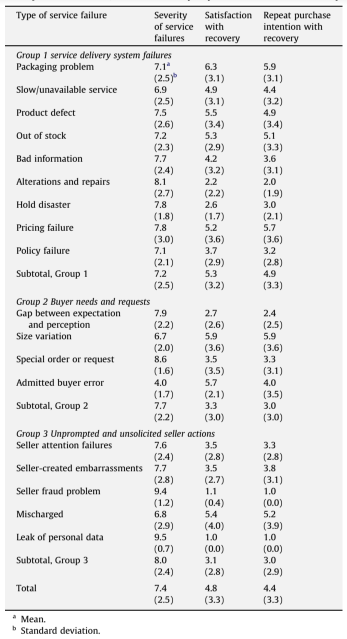
\includegraphics[height=.5\textheight]{images/bab3/Fatalitas-Kegagalan-Ecommerce.png}
        \caption{Fatalitas kegagalan dalam aplikasi Lelang Online, Kepuasan terhadap Perbaikan Pelayanan dan \textit{Repeat Purchase Intention} setelah Perbaikan Layanan}
        \label{severity-failures}
      \end{figure}
      
      \indent Dalam gambar diatas, dijabarkan beberapa jenis kegagalan yang pernah dialami oleh pengguna aplikasi serta fatalitas/pengaruh buruk kegagalan tersebut terhadap kepercayaan pengguna. 
      
	  \begin{figure}[H]
        \centering
        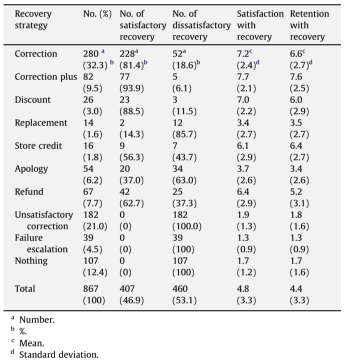
\includegraphics[width=\linewidth]{images/bab3/Solusi-Perbaikan-Ketidakpuasan.png}
        \caption{Kategori Perbaikan terhadap Kegagalan Pelayanan Lelang Online}
        \label{service-recovery-strategies}
      \end{figure}
      
      \indent Maka berdasarkan hasil analisa tersebut, fitur-fitur yang perlu ditambahkan selain daripada fitur dasar aplikasi lelang online adalah sebagai berikut :
      \begin{enumerate}
      \item Fitur chatting, untuk mengurangi kemungkinan \textit{Bad Information} dimana ekspektasi dan persepsi terhadap barang yang dilelang antara pembeli dan penjual tidak sama dan \textit{Special Needs}, 
      \item Fitur pemberian kupon voucher (\textit{Discount and Correction Plus}) yang bisa berupa \textit{free shipping} atau \textit{discount}.
      \end{enumerate}
   %checked
	\subsection{\textit{Bussiness Aspects of Software Engineering}}
	
	Lelang merupakan salah satu metode pertukaran barang dan jasa dengan metode penetapan harga yang berbeda dengan perdagangan. Oleh karena itu, lelang juga termasuk dalam kategori bisnis. Yang menarik adalah, ketika bisnis digabungkan dengan teknologi atau yang sering disebut \textit{e-commerce}, hal yang sekedar pertukaran barang bertransformasi menjadi sebuah sistem interaktif yang kompleks dimana tujuan utamanya adalah menarik pengunjung/pengguna untuk menyelesaikan sebuah transaksi. Hal ini tentu sangat krusial, penting, dan tertantang untuk menyelesaikannya. \\
	\indent Dalam mencapai kesuksesan dan tingkat kompetitif yang tinggi, haruslah menyediakan layanan dengan kesan \textit{user experience (UX)} yang positif bagi para penggunanya. Morville  \cite[p.~27]{a-set-of-heuristics-2014} , dalam studi yang dilakukannya, menyebutkan bahwa UX tercakup dalam 7 aspek esensial, yaitu \begin{enumerate}[label=\alph*.]
		\item \textit{useful}
		\item \textit{usable}
		\item \textit{findable}
		\item \textit{desirable}
		\item \textit{accessible}
		\item \textit{credible}.
		\end{enumerate}
	
	\indent Hasil-hasil temuan penting yang menarik dalam pengaruh \textit{user experience}, adalah sebagai berikut dikutip dari sebuah sumber adalah sebagai berikut:
	\begin{enumerate}[label=\alph*.]
		\item \textit{User tend to leave if a page loads more than 3 seconds};
		\item \textit{79\% of users won't return if the web's performance and experience is poor};
		\item \textit{44\% of users will tell the poor experiences to their friends}.
	\end{enumerate}
	
	\indent Selain dari faktor \textit{user experience} dan \textit{performance}, beberapa hal yang menjadi poin penting dan menarik dalam beberapa studi yang terkait adalah sebagai berikut:
	\begin{enumerate}[label=\alph*]
		\item \textit{Familiarity} - yang dapat didefinisikan sebagai tingkat familier atau kesamaan dengan sistem sejenis ternyata dapat membangun \textit{trust} sehingga mensugesti pengguna untuk menyelesaikan transaksi yang dilakukan;
		\item \textit{Usability} yang memudahkan pengguna dalam menyelesaikan transaksi; dan
		\item Aspek-aspek psikologi seperti pemilihan warna, penggunaan \textit{icon} yang sesuai, seperti \textit{icon} gembok pada halaman pembayaran ternyata dapat mengesankan \textit{security} pada pengguna.
	\end{enumerate}
	
	
	\begin{figure}[H]
		\centering
		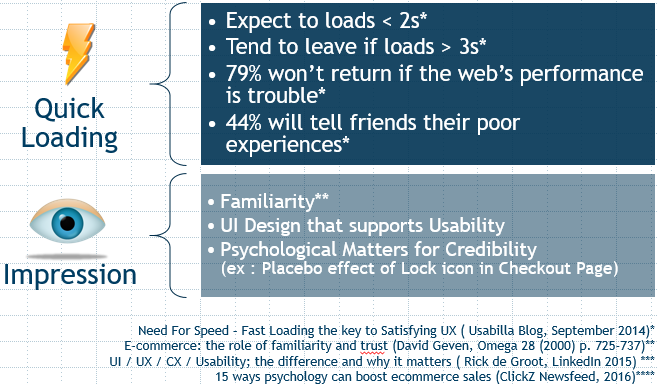
\includegraphics
		[width=\textwidth]
		{images/bab3/analisa/user-centered.png}
		\caption{Visualisasi aspek bisnis dalam \textit{software engineering}}
		\label{user-centered-analysis}
	\end{figure}
	
	\indent Dari hasil temuan ini, dapat disimpulkan bahwa \textit{user experiences, performances, usability} dan psikologi memiliki pengaruh besar dalam kesuksesan lelang online dalam menarik hati para penggunanya. Hal ini akan mempengaruhi definisi kebutuhan fungsionalitas yang akan dibahas dalam subbab \ref{keb-fungsional}.
		
		
		 
	  \subsubsection{Spesifikasi Kebutuhan Fungsional}
  \label{keb-fungsional}
	Berdasarkan deskripsi umum sistem pada subbab \ref{deskripsi-umum-app}, maka dapat disimpulkan bahwa kebutuhan fungsional dari aplikasi lelang online, yang dipaparkan dalam Tabel \ref{tabel-fungsional}.

  \LTXtable{\textwidth}{tables/03b/functional.tex}	
   %checked
	
  \subsection{Spesifikasi Kebutuhan Non-Fungsional}
  
  Kebutuhan non-fungsional yang harus dipeuhi oleh aplikasi ini berhubungan dengan faktor-faktor sebagai berikut:

	\LTXtable{\textwidth}{tables/03b/nonfunctional.tex}	
  
  \newpage %checked
	\subsubsection{\textit{Bussiness Modelling Workflow}} 
	\subsection{Spesifikasi Kasus Penggunaan}
	Kasus penggunaan disini dimaksudkan untuk menurunkan kebutuhan fungsional yang telah dispesifikasikan sebelumnya pada tabel \ref{tabel-fungsional} sebelumnya.\\
	Daftar kasus Penggunaan dapat dilihat pada \ref{kasus-penggunaan}.
	
	\LTXtable{\textwidth}{tables/03c/kasus_penggunaan.tex}
	\begin{figure}[H]
		\centering
		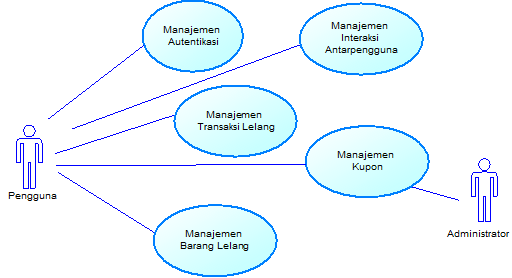
\includegraphics
		[width=\textwidth]
		{images/bab3/usecasediagram/ucd-main.png}
		\caption{Diagram Kasus Penggunaan Aplikasi}
		\label{ucd.main}
	\end{figure}
	
	Selanjutnya, akan dijabarkan masing-masing Spesifikasi Kasus Penggunaan untuk semua  Kasus Penggunaan yang telah dijabarkan diatas.
	
	\subsubsection{KP01. Manajemen Authentikasi Pengguna}

	Pada kasus penggunaan ini, pengguna dapat memanajemen autentikasi dan pendaftaran ke dalam sistem.\\

	% Login
	\input{Chapters/Details/bab3/3cxx/01/01}
	
	% Registrasi
	\input{Chapters/Details/bab3/3cxx/01/02}
	
	% Konfirmasi Email
	\input{Chapters/Details/bab3/3cxx/01/03}
	
	\subsubsection{KP02. Manajemen Transaksi Lelang}
\label{kp02}

Pada kasus penggunaan ini, pengguna akan dapat memanajemen transaksi dan penawaran-penawaran yang ia berikan terhadap barang yang terdaftar dalam alikasi.\\

	% Melihat daftar barang yang dilelang
	\input{Chapters/Details/bab3/3cxx/02/01}
	
	% Mencari barang yang diinginkan
	\input{Chapters/Details/bab3/3cxx/02/02}
	
	% Menawar/melelang barang
	\input{Chapters/Details/bab3/3cxx/02/03}
	
	% Melihat riwayat transaksi penawaran harga terhadap barang
	\input{Chapters/Details/bab3/3cxx/02/04}
	
	\subsubsection{KP03. Manajemen Barang Lelang}
\label{kp03}

Pada kasus penggunaan ini, pengguna akan dapat memanajemen barang yang ia daftarkan untuk dilelang, dan melihat proses monitoringnya, seperti yang dipaparkan pada penjelasan berikut.\\

% Mendaftarkan barang untuk dilelang
\input{Chapters/Details/bab3/3cxx/03/01}

% Memperbarui informasi barang yang dilelang
\input{Chapters/Details/bab3/3cxx/03/02}

% Melihat barang yang pernah didaftarkan
\input{Chapters/Details/bab3/3cxx/03/03}

% Melihat riwayat harga yang ditawarkan pada barang yang dilelang
\input{Chapters/Details/bab3/3cxx/03/04}
	
	\subsubsection{KP04. Manajemen Interaksi Antarpengguna}
\label{kp04}
	\begin{figure}[H]
		\centering
		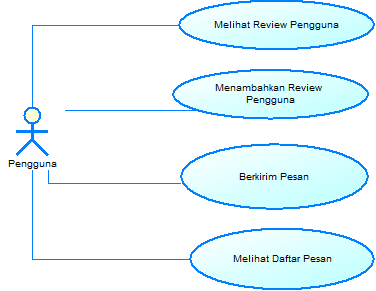
\includegraphics
		[width=\textwidth]
		{images/bab3/usecasediagram/ucd-04.png}
		\caption{Diagram Kasus Penggunaan Manajemen Interaksi Antarpengguna}
		\label{ucd.04}
	\end{figure}
Pada kasus penggunaan ini, pengguna difasilitasi untuk berinteraksi, memberikan \textit{review}/testimoni terhadap pengguna lainnya sesuai dengan keinginan.

	% Melihat review pengguna
	\input{Chapters/Details/bab3/3cxx/04/01}
	
	% Menambahkan Review Pengguna
	\input{Chapters/Details/bab3/3cxx/04/02}
		
	% Berikirim pesan
	\input{Chapters/Details/bab3/3cxx/04/04}

	% Melihat daftar pesan
	\input{Chapters/Details/bab3/3cxx/04/05}
	
%	\subsubsection{KP05. \textit{Monitoring} Proses Lelang}
\label{kp05}
	\begin{figure}[H]
		\centering
		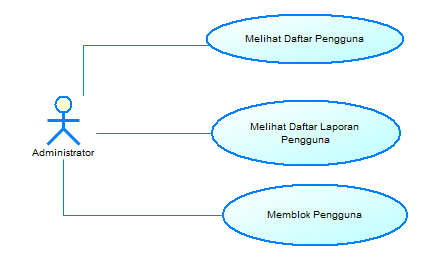
\includegraphics
		[width=\textwidth]
		{images/bab3/buku/usecasediagram/ucd-05.png}
		\caption{Diagram Kasus Penggunaan \textit{Monitoring} Lelang}
		\label{ucd.05}
	\end{figure}
Kasus penggunaan ini seluruhnya digunakan oleh \textit{administrator} aplikasi, dan dilakukan di sistem terpisah.

% Melihat daftar pengguna
\input{Chapters/Details/bab3/3cxx/05/01}

% Melihat daftar laporan pengguna
\input{Chapters/Details/bab3/3cxx/05/02}

% Memblock pengguna
\input{Chapters/Details/bab3/3cxx/05/03}
	
	\subsubsection{KP05. Manajemen Voucher}
\label{kp05}

	\begin{figure}[H]
		\centering
		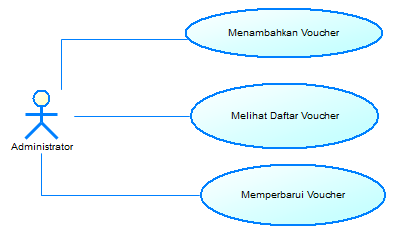
\includegraphics
		[width=\textwidth]
		{images/bab3/usecasediagram/ucd-06.png}
		\caption{Diagram Kasus Penggunaan Manajemen Kupon}
		\label{ucd.06}
	\end{figure}
	Kasus penggunaan ini seluruhnya digunakan oleh \textit{administrator} aplikasi dan dilakukan di sistem terpisah. Kasus penggunaan ditujukan untuk mempermudah \textit{administrator} dalam memanajemen voucher/kupon yang dibagikan oleh pengguna.

	% Menambahkan voucher
	\input{Chapters/Details/bab3/3cxx/06/01}
	
	% Melihat daftar voucher
	\input{Chapters/Details/bab3/3cxx/06/02}
	
	% Memperbarui Voucher
	\input{Chapters/Details/bab3/3cxx/06/03}







 %checked
	
	
	%Technical Analysis
	\subsection{\textit{Technical Analysis}}
	\subsection{Identifikasi Komponen Fundamental}
	Berdasarkan Bab Analisa, dapat diidentifikasi dan divisualisasikan pada Gambar \ref{fundamental-component} yaitu komponen-komponen penting dalam pembuatan aplikasi sebagai berikut:
	\begin{enumerate}
		\item Web Server 
		\item Mekanisme penyimpanan data (\textit{database} dan \textit{data storage})
		\item \textit{User Interface} sebagai media terhadap \textit{end-user}
		\item Mekanisme Asinkronus untuk mengakomodasi fitur \textit{realtime}
	\end{enumerate}
	
	\begin{figure}[H]
		\centering
		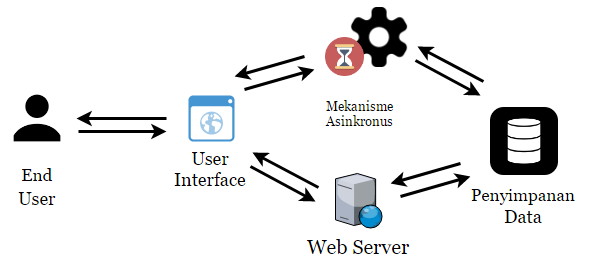
\includegraphics
		[width=\textwidth]
		{images/bab3/buku/basic_architecture.png}
		\caption{Arsitektur dasar yang dibutuhkan untuk membangun aplikasi}
		\label{fundamental-component}
	\end{figure}
	
	
	

	\subsection{\textit{Arsitektur Fundamental}}
	
\subsection{\textit{Technology Options}}
\label{tech-options}

	Pada subbab sebelumnya, penulis sudah memaparkan arsitektur dasar yang dibutuhkan dalam rancang bangun aplikasi. Terkait dengan arsitektur dasar tersebut, banyak pilihan teknologi yang dapat mengimplementasikan arsitektur tersebut. Dalam pemaparan selanjutnya, akan dijelaskan alasan penulis \textit{best practice} dalam pemilihan teknologi yang digunakan, didasarkan pada \textit{best practices} dan pengalaman-pengalaman penulis. Keterkaitan dengan aspek-aspek yang dijelaskan sebelumnya pada subbab \ref{tech-analysis}.
	
	\subsubsection{\textsc{Nginx} sebagai Web Server}
		\begin{itemize}
			\item Kelebihan
				\begin{enumerate}
					\item Konfigurasi yang lebih \textit{friendly} dan terstruktur
					\item Ketersediaan fitur yang lengkap \& krusial (\textit{reverse proxy}, memungkinkan skalabilitas \& \textit{load balancing})
					\item \textit{Learning-gap} yang kecil terhadap pengalaman penulis/sudah familiar
				\end{enumerate}
			\item Opsi lainnya
				\begin{enumerate}
					\item Apache2:  Fiturnya kurang lengkap
					\item Node.js:  \textit{Learning-gap} yang besar bagi penulis/belum familiar
					\item Python:  Belum Familiar, dan perlu eksplorasi fitur lebih dalam
				\end{enumerate}
		\end{itemize}
	
	\subsubsection{\textsc{PostgreSQL} untuk Penyimpanan Data}
	\begin{itemize}
		\item Kelebihan
		\begin{enumerate}
			\item \textit{Learning gap} yang kecil
			\item Stabil karena telah digunakan dan dikembangkan oleh banyak \textit{developer} selama bertahun-tahun
		\end{enumerate}
		\item Opsi lainnya
		\begin{enumerate}
			\item SQL Server:  Instalasi yang kompleks, penggunaan \textit{resource} yang cukup besar
		\end{enumerate}
	\end{itemize}
	
	\subsubsection{\textsc{MongoDB} untuk Penyimpanan Data Nontansaksional}
		\begin{itemize}
			\item Kelebihan
			\begin{enumerate}
				\item \textit{Learning curve} yang mudah/sintaksnya kurang lebih sama dengan sintaks \textit{database} transaksional pada umumnya
				\item Performa yang cepat karena menggunakan BSON
				\item Fitur yang lengkap untuk \textit{sustainability} aplikasi seperti (Replikasi, Sharding, dll)
				\item \textit{Handling} terhadap data yang sangat besar yang cukup bagus, cocok untuk data yang masif seperti \textit{chatting}.
			\end{enumerate}
			\item Opsi lainnya
			\begin{enumerate}
				\item Redis:  Cepat, namun penyimpanan dilakukan di RAM sehingga lebih cocok untuk penyimpanan \textit{auth session}, bukan untuk penyimpanan data yang sifatnya masif
				\item Cassandra:  \textit{Learning-gap} yang besar, namun fiturnya lengkap untuk \textit{data mining}
			\end{enumerate}
		\end{itemize}
		
		
	\subsubsection{\textsc{CDN} sebagai \textit{Assets Sources}}
		\begin{itemize}
			\item Kelebihan
			\begin{enumerate}
				\item Akses cepat karena besar kemungkinan asset tersebut telah di\textit{cache} sebelumnya dalam browser pengguna
				\item Mengurangi \textit{bandwith} server
				\item Telah dioptimasi oleh pengembang masing-masing asset.
			\end{enumerate}
			\item Opsi lainnya
			\begin{enumerate}
				\item Disimpan dalam server: Mengurangi \textit{bandwith} server (\textit{cost} meningkat)
			\end{enumerate}
		\end{itemize}
		
	\subsubsection{\textsc{AWS S3} untuk \textit{Content Growth Scalability}}
	\begin{itemize}
		\item Kelebihan
		\begin{enumerate}
			\item \textit{Benefit} yang sangat \textit{krusial}:  keamanan, skalabilitas, \textit{availability} - karena sudah di\textit{handle} langsung oleh pengembang \textit{cloud computing} yang ahli di bidangnya
			\item Perkembangan jumlah konten yang akan disimpan (gambar barang yang diupload pengguna)  tentunya bersifat sangat masif, sehingga tidak mungkin disimpan dalam server
		\end{enumerate}
		\item Opsi lainnya
		\begin{enumerate}
			\item Disimpan dalam server: Mengurangi performa server karena sifatnya yang memakan \textit{resource} cukup banyak, dan menambah \textit{cost} untuk \textit{upgrade server storage}
		\end{enumerate}
	\end{itemize}
	
	\subsubsection{\textsc{SendGrid} untuk SMTP Relay}
	\begin{itemize}
		\item Kelebihan
		\begin{enumerate}
			\item Konfigurasi yang mudah
			\item Dokumentasi yang cukup lengkap dan mudah ditemukan
			\item Fitur yang lengkap
			\item Adanya \textit{free storage} dari akun Github Student Pack penulis
		\end{enumerate}
		\item Opsi lainnya
		\begin{enumerate}
			\item MailChimp:  Dokumentasi kurang lengkap, tidak ada \textit{free storage} untuk akun penulis
		\end{enumerate}
	\end{itemize}
	
	\subsubsection{\textsc{Vue.js} untuk \textit{Workloads Sharing}}
		\begin{itemize}
			\item Kelebihan
			\begin{enumerate}
				\item \textit{Learning-gap} relatif kecil dibandingkan \textit{Javascript tools} lainnya, karena didesain khusus untuk Laravel
				\item Adanya program utilitas (webpack) yang membuat performa Vue.js jauh lebih cepat
				\item Logika aplikasi dapat di\textit{obfuscate} dengan webpack (\textit{embedded} dalam Laravel)
			\end{enumerate}
			\item Opsi lainnya
			\begin{enumerate}
				\item React:  \textit{Learning gap} dan \textit{learning curve} yang sangat besar untuk penulis
				\item jQuery:  tidak efektif karena \textit{code smells} yang ditimbulkan cukup banyak
			\end{enumerate}
		\end{itemize}
		
	\subsubsection{\textsc{Socket.io} untuk Mekanisme Asinkronus}
		\begin{itemize}
			\item Kelebihan
			\begin{enumerate}
				\item \textit{Learning-gap} relatif kecil dibandingkan \textit{Javascript tools} lainnya, karena didesain khusus untuk Laravel
				\item Adanya program utilitas (webpack) yang membuat performa Vue.js jauh lebih cepat
				\item Logika aplikasi dapat di\textit{obfuscate} dengan webpack (\textit{embedded} dalam Laravel)
			\end{enumerate}
			\item Opsi lainnya
			\begin{enumerate}
				\item React:  \textit{Learning gap} dan \textit{learning curve} yang sangat besar untuk penulis
				\item jQuery:  tidak efektif karena \textit{code smells} yang ditimbulkan cukup banyak
			\end{enumerate}
		\end{itemize}		
		
	\subsubsection{\textsc{JWT} untuk Keamanan Soket}
		\begin{itemize}
			\item Kelebihan
			\begin{enumerate}
				\item \textit{Library support} yang lengkap untuk komponen-komponen lainnya
				\item Efektif dan efisien karena tidak ada \textit{query} ke database untuk autentikasi
			\end{enumerate}
			\item Opsi lainnya
			\begin{enumerate}
				\item \textit{Query} ke \textit{database} secara konvensional:  Sifat koneksi soket yang masif akan sangat memberatkan \textit{database} jika setiap kali ada koneksi baru, harus melakukan \textit{query database} sehingga tidak efektif
				\item \textit{Session caching} dengan Redis:  \textit{Learning gap} yang besar
			\end{enumerate}
		\end{itemize}
		
	\subsubsection{\textsc{Laravel Dusk} untuk \textit{Functionality Testing Script}}
		\begin{itemize}
			\item Kelebihan
			\begin{enumerate}
				\item \textit{Learning gap} yang kecil karena didesain sefamiliar mungkin dengan Laravel
			\end{enumerate}
			\item Opsi lainnya
			\begin{enumerate}
				\item Selenium:  \textit{Learning curve} yang besar
				\item Phantom.js:  \textit{Learning curve} yang besar
			\end{enumerate}
		\end{itemize}
	
	

	
	
	
	\subsection{\textit{Summary}}



\subsection{Analisa \textit{User Experience} dari E-Commerce di Indonesia}
\label{alasan-ux-ecommerce-indonesia alasan-app-serupa}
Selama masa pengerjaan aplikasi, penulis sering menganalisa dan memperhatikan kebiasaan-kebiasaan yang umum di website \textit{e-commerce} di Indonesia. Salah satu yang paling sering dianalisa oleh penulis adalah adalah situs Tokopedia.
\\
\indent Beberapa hal yang dianalisa penulis adalah:
\begin{enumerate}
	\item Halaman yang muncul bukanlah eagerloading, tapi \textit{lazy loading}\\
	\indent Ini adalah solusi cerdas untuk mengakali \textit{delay loading item} yang sudah pasti jumlahnya sangat banyak (maka butuh \textit{query} yang tentunya memakan waktu cukup lama), namun juga memainkan faktor psikologi / \textit{user behaviour} pengguna dengan membiarkan pengguna melihat tahap demi tahap halaman 'diisi'.
	\item \textit{User Interface} yang sederhana dan pemilihan warna yang \textit{soft}
\end{enumerate}
Dari 2 poin tersebut, sebisa mungkin saya adaptasi ke dalam aplikasi Lelang Online ini.

\subsection{Analisa Keamanan pada koneksi Soket}
\label{alasan-socket.io}
Untuk mengakomodasi fitur yang bersifat \textit{realtime}, dibutuhkan koneksi ke soket secara terus menerus. Hal ini tentu dapat menjadi sasaran empuk \textit{security} karena jika tidak diamankan, maka dapat menjadi peluang besar bagi para pihak yang tidak berkepentingan untuk merusak proses bisnis aplikasi.\\
\indent Namun, jika dalam setiap koneksi soket harus mengirimkan \textit{credentials}, hal ini tentu menjadi tidak praktis dan malah lebih berbahaya karena membiarkan data-data sensitif seperti \textit{password} dan \textit{username} berlalu-lalang di jaringan internet. Selain itu, \textit{disadvantage}nya adalah ketidakpraktisan untuk selalu meng\textit{query} database setiap kali ada koneksi, tentu saja ini memperlambat kerja \textit{database} dan menambah waktu \textit{delay}.\\
\indent Untuk menyiasatinya, penulis menerapkan JWT.io dengan keuntungan sebagai berikut :
\begin{enumerate}
	\item Tidak perlu \textit{query} ke database karena hanya menggunakan security token yang di\textit{generate} dengan formula tertentu
	\item Tidak perlu ada aplikasi khusus yang menjembatani aplikasi Soket dan aplikasi WebServer - sehingga lebih praktis
	\item Data-data sensitif menjadi lebih terjaga karena tidak perlu dipertukarkan setiap koneksi ke soket.
\end{enumerate}

\subsection{Analisa \textit{Best Practice} dalam Struktur Perangkat Lunak}
\label{alasan-best-practice}
Pada dasarnya, Laravel adalah kerangka kerja MVC. Namun, ada banyak fitur yang ada dalam aplikasi Lelang Online ini yang tidak terakomodasi dalam MVC, misal sebagai berikut :
\begin{enumerate}
	\item Sistem Verifikasi lewat Email - yang berarti aplikasi harus berinteraksi dengan SMTP server
	\item Sistem \textit{Generate} Token JWT.io, dimana dalam proses \textit{Generate Token} sama sekali tidak ada database dilibatkan.
\end{enumerate}

\indent Jika fitur-fitur tersebut 'dipaksa' dimuat ke dalam MVC, maka tentu saja strukturnya menjadi ganjil, dan muncul \textit{code smell} berikut :
\begin{enumerate}
	\item \textit{Large Class}, dimana terdapat satu buah file yang sangat panjang (biasanya merupakan entitas utama, dalam hal ini contohnya barang/\textit{item})
	\item \textit{Inappropriate Intimacy}, dimana terdapat satu kelas yang menyimpan \textit{logic} yang tidak seharusnya ia simpan
	\item \textit{Duplicated Code}
\end{enumerate}

\indent Untuk menghindari kemungkinan \textit{code smell} tersebut, maka penulis menyiasatinya dengan cara berikut :
\begin{enumerate}
	\item Penggunaan Repository Pattern
	\\ Memisahkan antara Data Processing Layer dan View Layer - agar lebih rapi, terstruktur, hal ini juga dapat menghindari \textit{Duplicated Code}.
	\item Penambahan Komponen : Service dan Provider \\
	Untuk memisahkan \textit{logic} aplikasi yang terkait dengan akses pihak ketiga. Tujuannya, agar jika kedepannya terdapat perbaikan fitur/penambahan fitur, lebih mudah melakukan \textit{traceback} terhadap file/kelas yang bertanggungjawab terhadap fitur tersebut.
\end{enumerate}

\subsection{Analisa Aplikasi Serupa}
\label{alasan-app-serupa}
Selama pengerjaan aplikasi, penulis menganalisa aplikasi serupa. Penulis menemukan aplikasi yang kurang lebih alur bisnis / alur penggunaan aplikasinya serupa yaitu : Carousell. \\
\indent Penulis melihat ada beberapa kesamaan antara sifat transaksi aplikasi tugas akhir saya dengan aplikasi tersebut, yaitu :
\begin{enumerate}
	\item Sama-sama tidak mengakomodasi pembayaran
	\item Sama-sama tidak adanya kepastian harga (bedanya, pada Carousell yang terjadi adalah \textit{bargaining}
\end{enumerate}
\indent Sehingga dalam alur proses nya, banyak diadaptasi dari Carousell, agar pengguna dapat lebih familiar dan \textit{predictability}nya lebih tinggi jika diadaptasi dari \textit{E-commerce} lainnya yang lebih umum digunakan oleh pengguna.
  
  \pagebreak
  \section{Spesifikasi Kebutuhan dan Pengguna}
   
  \subsection{Deskripsi Umum}
  
  Pada bagian ini membahas garis besar aplikasi secara umum, menjabarkan fitur-fitur penting yang dijelaskan dari subbab sebelumnya.  
  \begin{enumerate}
  \item \textbf{Registrasi ke dalam sistem}
    \item \textbf{Login ke dalam sistem}
    \item \textbf{Mendaftarkan barang untuk dilelang} \\
        Pengguna dapat mendaftarkan barangnya untuk dijual dan dilelang. Selain itu, pengguna dapat menentukan harga awal dan batas waktu lelang pada saat mendaftarkan barangnya.
    \item \textbf{Memperbarui barang yang dilelang} \\
        Pengguna dapat memperbarui informasi mengenai barang yang dilelang, seperti nama barang, menambah foto deskripsi barang, atau menambah waktu lelang.
    \item \textbf{Melihat informasi barang yang dilelang} \\
        Pengguna dapat melihat detail informasi barang yang sedang dilelang – seperti foto barang, riwayat penawaran harga barang lelang, sisa waktu penawaran, deskripsi barang, dsb.
    \item \textbf{Melihat informasi riwayat lelang} ( Siapa saja yang sudah mengajukan penawaran dan harga yang ditawarkan )
    \item \textbf{Mengajukan penawaran harga untuk barang yang dilelang / Menjadi auctioneer} \\
        Selain menjadi auctioneer, pengguna juga dapat menawarkan harga terhadap barang-barang yang didaftarkan oleh pengguna lain.
    \item \textbf{Mendapatkan pemberitahuan jika penawaran harga dikalahkan dengan harga lebih tinggi} \\
        Pengguna mendapatkan pemberitahuan jika pengguna sedang mengikuti pelelangan barang, dan ada penawaran harga yang lebih tinggi dari penawaran oleh pengguna tersebut, sehingga pengguna dapat mengikuti perkembangan harga dari barang yang dilelang.
    \item \textbf{Mengikuti / follow barang yang sedang dilelang dan mendapatkan pemberitahuan jika barang tersebut }\\
        Jika pengguna sedang tidak ingin melelang barang namun ingin tetap mengetahui informasi dari suatu barang lelang, pengguna dapat mengikuti feed/berita dari barang tersebut.
    \item \textbf{Mendapatkan pemberitahuan jika memenangkan lelang atau tidak.}\\
        Jika pengguna mengajukan penawaran harga terhadap suatu barang, maka pengguna akan mendapatkan pemberitahuan pada saat batas waktu lelang selesai, apakah pengguna tersebut memenangkan proses lelang tersebut atau tidak.
    \item \textbf{Saling berkirim pesan singkat/chat kepada auctioneer/penawar harga }\\
        Untuk saling bertukar informasi mengenai barang yang sedang dilelang, auctioneer dan penawar harga dapat saling berkirim pesan singkat.
    \item \textbf{Melihat riwayat penawaran harga lelang }\\
        Pengguna dapat melihat barang riwayat penawaran harga yang diberikan oleh pengguna tersebut terhadap semua barang yang pernah dia lelang.
    \item \textbf{Melihat riwayat barang yang dilelang }\\
        Pengguna dapat melihat riwayat barang yang pernah ditawar harganya/diberikan penawaran harga.
    \item \textbf{Memberi review tentang pengguna lain sebagai auctioneer dan atau sebagai penawar harga }\\
        Pengguna dapat memberikan komentar/testimoni berdasarkan pengalaman bertransaksi/penawaran harga dengan pengguna lainnya, baik pengalaman memuaskan ataupun pengalaman buruk.
    \item\textbf{ Melihat review mengenai seorang pengguna }\\
        Selain memberikan review, pengguna dapat melihat review seorang pengguna.
    \item \textbf{Memblok pengguna sebagai auctioneer }\\
        Auctioneer dapat memblok pengguna agar pengguna tersebut tidak memberikan penawaran harga terhadap barang yang sedang ia lelang. Hal ini bisa saja karena review/testimoni pengguna tersebut buruk atau karena alasan lainnya.
    \item \textbf{Mencari barang yang dilelang dengan keyword tertentu}
  \end{enumerate}
  
  \subsection{Spesifikasi Kebutuhan Fungsional}
  \vspace{-5mm}
  Berdasarkan deskripsi umum aplikasi, kebutuhan fungsional dari aplikasi dijabarkan di \cref{tabel-fungsional} .
  
\begin{table}[H]
\centering
\resizebox{\columnwidth}{!}{%
\begin{tabular}{|p{0.1\columnwidth}|p{0.3\columnwidth}|p{0.6\columnwidth}|}
\hline
\multicolumn{1}{|c|}{\textbf{No.}} & \multicolumn{1}{c|}{\textbf{\begin{tabular}[c]{@{}c@{}}Kebutuhan \\ Fungsional\end{tabular}}} & \multicolumn{1}{c|}{\textbf{Deskripsi}} \\ \hline
1 & Manajemen Akun & Pengguna :Memperbarui dan mengubah informasi pengguna dalam akun \\ \hline
2 & Memanajemen penawaran terhadap barang lelang & Pengguna :Menawar barang, mendapat informasi barang, mencari barang yang diinginkan, dan fitur-fitur yang mempermudah pengguna dalam penawaran barang \\ \hline
3 & Memanajemen barang yang dilelang & Pengguna :Mendaftarkan barang untuk dilelang, melihat progress kemajuan lelang, membatalkan lelang dari pengguna tertentu \\ \hline
4 & Memanajemen Laporan Pengguna & Pengelola : Melihat daftar laporan dari pengguna, memblokir pengguna yang melanggar ketentuan \\ \hline
5 & Memanajemen Kupon & Pengelola : Membuat kupon, melihat daftar kupon, melihat riwayat penggunaan kupon \\ \hline
\end{tabular}%
}
\caption{Kebutuhan Fungsional Aplikasi Lelang Online}
\label{tabel-fungsional}
\end{table}
  
  \subsection{Spesifikasi Kebutuhan Non-Fungsional}
  
  Kebutuhan non-fungsional yang harus dipeuhi oleh aplikasi ini berhubungan dengan faktor-faktor sebagai berikut :

\begin{table}[H]
\centering
\resizebox{\columnwidth}{!}{%
\begin{tabular}{|p{0.1\columnwidth}|p{0.3\columnwidth}|p{0.6\columnwidth}|}
\hline
\textbf{No} & \multicolumn{1}{c|}{\textbf{Parameter}} & \multicolumn{1}{c|}{\textbf{Ketersediaan}}                             \\ \hline
 1  & Ketersediaan & Aplikasi harus dapat berjalan pada browser , tanpa dibatasi waktu dan tempat selama browser tersebut tersambung ke jaringan internet. \\ \hline
 2 & Bahasa & Bahasa yang digunakan pada antarmuka merupakan bahasa Indonesia \\ \hline
3 & Otorisasi & Setiap pengguna dilengkapi dengan akses \\ \hline
4 & Portabilitas & Aplikasi dapat diakses pada semua platform selama platform tersebut terinstall web browser \\ \hline
\end{tabular}
}
\caption{Kebutuhan Non-Fungsional Aplikasi Lelang Online}
\label{tabel-non-fung}
\end{table}
  
  \newpage
  
  \subsection{Identifikasi Pengguna}
  Pengertian pengguna adalah pihak-pihak, baik manusia maupun sistem atau perangkat lain yang terlibat dan berinteraksi secara langsung dengan sistem. Pada aplikasi lelang online ini, terdapat dua pengguna yaitu pengguna dan pengelola / \textit{administrator}. Detail tugas dan hak akses pengguna dapat dilihat pada Tabel \ref{tugas-hak-akses} berikut.
  
\begin{table}[H]
\centering
\resizebox{\columnwidth}{!}{%
\begin{tabular}
{|p{0.1\columnwidth}|p{0.3\columnwidth}|p{0.3\columnwidth}|p{0.3\columnwidth}|}
\hline
\multicolumn{1}{|c|}{\textbf{Kategori Pengguna}} & \multicolumn{1}{c|}{\textbf{Tugas}} & \multicolumn{1}{c|}{\textbf{\begin{tabular}[c]{@{}c@{}}Hak Akses\\ ke Aplikasi\end{tabular}}}                                 

& \multicolumn{1}{c|}{\textbf{\begin{tabular}[c]{@{}c@{}}Kemampuan yang\\ Harus Dimiliki\end{tabular}}}                         \\ \hline
Pengguna                                         & Pelaku lelang & Fitur-fitur lelang & Pengetahuan dasar lelang, pengetahuan dasar untuk mengakses aplikasi berbasis web \\ \hline
Pengelola & Pengawas jalannya lelang & Fitur-fitur administrator seperti menambahkan kupon, memblokir pengguna, melihat daftar laporan pengguna  & Pengetahuan dasar lelang                                     
\\ \hline
\end{tabular}
}
\caption{Detail Tugas dan Hak Akses Pengguna}
\label{tugas-hak-akses}
\end{table}
  
  
  
  \pagebreak
  \section{Perancangan Sistem}



  
\subsection{Perancangan \textit{Data Sources dan Data Storage}}

	Untuk penyimpanan data, terdapat 2 jenis data yang sifatnya cukup berbeda, yaitu sebagai berikut :
    \\
    
    \begin{enumerate}
    \item \textbf{Data Transaksional disimpan di DBMS SQL - \textit{Relational}}
    \newline
    Data yang sifatnya \textit{transaksional}, seperti data \textit{bidding}, data pengguna, dan lain sebagainya.
    Untuk data ini, lebih baik jika menggunakan database Postgre, untuk menjaga integritas data dan \textit{integrity checking} juga  menjadi lebih mudah.
    \newline
    
    \item 
    \textbf{Data Non-Transaksional disimpan di DBMS NoSQL}
    \newline
    Seperti data \textit{chatting}, data \textit{joined rooms} tidak cocok dimasukkan kedalam database transaksional karena sifat pertambahan datanya yang sangat cepat dan urgensi integritas data tidak terlalu diprioritaskan (dibanding dengan data transaksional pada poin sebelumnya.
    \newline
    Oleh karena itu, baiknya data ini disimpan pada database NoSQL - pada rancang bangun aplikasi ini, DBMS NoSQL yang digunakan adalah MongoDB.
    \newline
    
    
    \item \textbf{Data Citra/Gambar disimpan di \textsc{Amazon Web Services}} \newline
    Gambar-gambar barang yang didaftarkan untuk dilelang, disimpan di \textit{cloud} dengan menggunakan \textit{Amazon Web Services}. Alasan-alasan menggunakan AWS sebagai data storage untuk gambar adalah sebagai berikut :
        \begin{enumerate}[noitemsep,topsep=0pt]
        \item Skalabilitas aplikasi lebih terjaga. 
        \newline Dengan memisahkan penyimpanan antara gambar dan server sehingga lebih mudah me\textit{maintain} perkembangan aplikasi, dan lebih fokus terhadap pengembangan aplikasi.
        \item Menyediakan \textit{built-in} keamanan, fleksibel dan efisiensi \cite{wikipedia_amazon_2016}
        \item Mencoba belajar menggunakan Amazon Web Services
        \end{enumerate}
        
    \item \textbf{Data \textit{Assets} Website}
    \newline
    Untuk data \textit{assets} yang dibutuhkan untuk website, terdapat beberapa kriteria penyimpanan berikut
    
      \begin{itemize}[noitemsep,topsep=0pt]
      \item Jika file tersebut sudah umum digunakan dan terdapat file CDNnya, maka akan akses CDNnya
      \newline
      Hal ini dimaksudkan agar \textit{loading} lebih cepat, sesuai dengan yang tercantum pada sumber \cite{sitepoint_7_2011}
      \item Jika file tersebut merupakan \textit{custom asset}, \textit{asset} yang dikustomisasi khusus untuk aplikasi ini, maka asset tersebut akan disimpan dalam server.
      \end{itemize}
    
    \end{enumerate}
  
  \subsection{Perancangan Skema \textit{Database}}

	Pada awalnya, database didesain dengan PDM sebagai berikut berikut : 
	
	\begin{figure}[H]
		\centering
		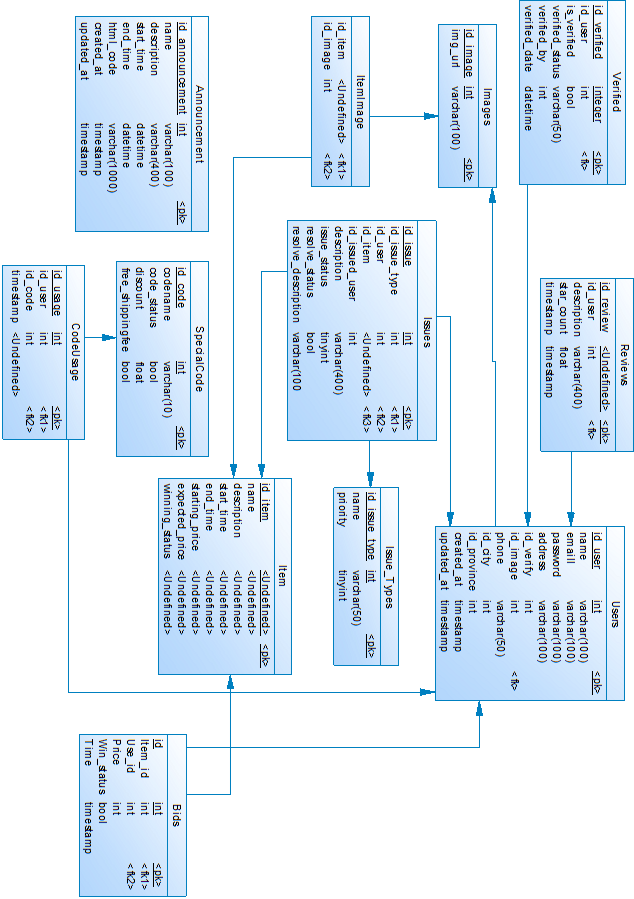
\includegraphics[height=0.6\paperheight]{images/bab3/db/pdm-awal.png}
		\caption{Rancangan Awal PDM untuk Database Relasional}
		\label{pdm-awal}
	\end{figure}
	
	Dan untuk tabel NoSQL dirancang sebagai berikut :
	\begin{figure}[H]
		\centering
		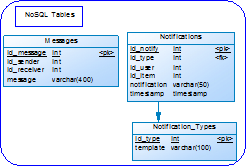
\includegraphics[width=\textwidth]{images/bab3/db/pdm-nosql-awal.png}
		\caption{Rancangan Awal PDM untuk Database Non-Relasional}
		\label{pdm-nosql-awal}
	\end{figure}
	
	Untuk database versi paling \textit{update}, dapat dilihat pada gambar berikut :
	\begin{figure}[H]
		\centering
		
\includegraphics[width=\textwidth]{images/no-image.png}
		\caption{PDM ter\textit{update} untuk Database Relasional}
		\label{pdm-final}
	\end{figure}
	
	Dan untuk tabel NoSQL dirancang sebagai berikut :
	\begin{figure}[H]
		\centering
		
\includegraphics[width=\textwidth]{images/no-image.png}
		\caption{PDM Ter\textit{Update} Database Non-Relasional}
		\label{pdm-nosql-final}
	\end{figure}
	
	Namun, karena pengembangan aplikasi yang bersifat \textit{agile} dan terus berubah karena perkembangan dan \textit{improvization} dari hasil analisa penulis, sifatnya menjadi sangat dinamis.\\

	Berikut akan dipaparkan spesifikasi dan penjelasan setiap tabel.
	\subsubsection{Spesifikasi Tabel User}
	
	\begin{table}[H]
		\centering
		\begin{tabular}{|r|l|l|l|}
			\hline
			\multicolumn{4}{|c|}{\textbf{Tabel items}} \\ \hline
			\textbf{Deskripsi} & \multicolumn{3}{l|}{Tabel ini menyimpan data XX YY ZZ} \\ \hline
			\textbf{Penyimpanan} & \multicolumn{3}{l|}{Transaksional / PostgreSQL} \\ \hline
			\textbf{\begin{tabular}[c]{@{}r@{}}Growth \\ Speed\end{tabular}} & \multicolumn{3}{l|}{\begin{tabular}[c]{@{}l@{}}(masih dipertimbangkan, tapi ini isinya \\ perhitungan/kalkulasi kasar perhitungan \\ penambahan data)\end{tabular}} \\ \hline
			\multicolumn{4}{|c|}{\textbf{Penjelasan Kolom Tabel User}} \\ \hline
			\multicolumn{1}{|l|}{No} & Nama Atribut & Tipe Data & Keterangan \\ \hline
			\begin{tabular}[c]{@{}r@{}}1\\ {[}PK{]}\end{tabular} & ID & INT & \begin{tabular}[c]{@{}l@{}}Autoincrement\\ oleh Sistem\end{tabular} \\ \hline
			2 & Name & varchar(255) & \begin{tabular}[c]{@{}l@{}}Diisi oleh\\ Pengguna\end{tabular} \\ \hline
			\begin{tabular}[c]{@{}r@{}}3\\ {[}FK{]}\end{tabular} & Category\_id & int & Diisi pengguna \\ \hline
			4 & Updated\_at & timestamp & \begin{tabular}[c]{@{}l@{}}Diisi oeh\\ Sistem\end{tabular} \\ \hline
		\end{tabular}
		\caption{Spesifikasi Tabel Z}
		\label{items-tab}
	\end{table}
	
	
		\subsubsection{Spesifikasi Tabel User}
		
		\begin{table}[H]
			\centering
			\begin{tabular}{|r|l|l|l|}
				\hline
				\multicolumn{4}{|c|}{\textbf{Tabel items}} \\ \hline
				\textbf{Deskripsi} & \multicolumn{3}{l|}{Tabel ini menyimpan data XX YY ZZ} \\ \hline
				\textbf{Penyimpanan} & \multicolumn{3}{l|}{Transaksional / PostgreSQL} \\ \hline
				\textbf{\begin{tabular}[c]{@{}r@{}}Growth \\ Speed\end{tabular}} & \multicolumn{3}{l|}{\begin{tabular}[c]{@{}l@{}}(masih dipertimbangkan, tapi ini isinya \\ perhitungan/kalkulasi kasar perhitungan \\ penambahan data)\end{tabular}} \\ \hline
				\multicolumn{4}{|c|}{\textbf{Penjelasan Kolom Tabel User}} \\ \hline
				\multicolumn{1}{|l|}{No} & Nama Atribut & Tipe Data & Keterangan \\ \hline
				\begin{tabular}[c]{@{}r@{}}1\\ {[}PK{]}\end{tabular} & ID & INT & \begin{tabular}[c]{@{}l@{}}Autoincrement\\ oleh Sistem\end{tabular} \\ \hline
				2 & Name & varchar(255) & \begin{tabular}[c]{@{}l@{}}Diisi oleh\\ Pengguna\end{tabular} \\ \hline
				\begin{tabular}[c]{@{}r@{}}3\\ {[}FK{]}\end{tabular} & Category\_id & int & Diisi pengguna \\ \hline
				4 & Updated\_at & timestamp & \begin{tabular}[c]{@	{}l@{}}Diisi oeh\\ Sistem\end{tabular} \\ \hline
			\end{tabular}
			\caption{Spesifikasi Tabel Z}
			\label{items-2tab}
		\end{table}
	
  
  \subsection{Perancangan Arsitektur Aplikasi}
	
      \begin{figure}[H]
        \centering
        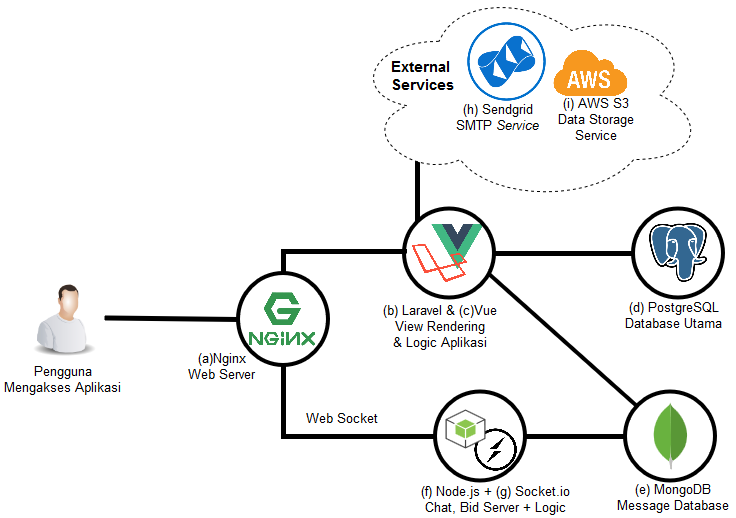
\includegraphics[width=\textwidth]{images/bab3/diagram/arsitektur-awal.png}
        \caption{Arsitektur Aplikasi Lelang Online 
        		\\
                \textit{External Services} artinya adalah menggunakan \textit{service} dari luar, tidak dibangun sendiri. }
        \label{arsitektur-app-final}
      \end{figure}
    
    \subsubsection{\textbf{\textsc{Nginx} sebagai WebServer dan Proxy Server}}
    {\scshape Nginx} adalah web server multifungsi - dimana selain berfungsi sebagai Webserver, namun juga bisa berfungsi sebagai Load Balancer. Dalam awal pembuatan aplikasi, \textsc{Nginx} hanya digunakan sebagai \textit{web server} untuk melayani permintaan halaman Web dari pengguna.
    \\
    Namun, saat \textit{deployment}, banyak sekali terjadi \textit{issue} yang berkaitan dengan \textit{ssl certificate}, sehingga pada akhirnya Nginx juga digunakan sebagai \textit{proxy server} - dimana Nginx mempunyai fungsi baru yaitu \textit{redirecting request=request} yang masuk ke dalam server, dan meneruskannya ke proses dalam server yang bertugas memproses \textit{request} tersebut.
	   \\
    Beberapa masalah yang ditemukan penulis, jika tidak menggunakan fitur \textsc{Nginx} sebagai proxy server untuk aplikasi Soket yang berbeda port adalah sebagai berikut :
	    \begin{itemize}[noitemsep,topsep=0pt]
	    \item CORS (Cross Origin Reference Source)
	    \newline
	    Dimana pada saat browser mengakses soket dari port lain (meskipun domainnnya sama), browser menganggap bahwa sambungan dari port lain tersebut sebagai \textit{security threat} dan otomatis memutuskan sambungan.
	    \item ERROR :: INSECURE RESPONSE!
	    \newline
	    Hal ini terjadi saat browser membuka sebuah web dengan https - namun mengakses koneksi soket yang tidak terproteksi dengan https. Hal ini juga membuat browser menganggap ini sebagai \textit{security threat}, dan tidak membuka \textit{reply} dari koneksi soket yang tidak terproteksi dengan https tersebut.
	    \end{itemize}
    
    \subsubsection {\textbf{Laravel dan Logika Aplikasi}}
    \textsc{Laravel}, bertugas sebagai Bos Besar, pengelola data dan manajemen data, dan pelayan \textit{request} dalam aplikasi Lelang online ini. Semua request diteruskan, dan diproses oleh \textsc{Laravel}, dan diproses oleh Laravel. 	    
    
    \subsubsection{\textbf{Vue.js sebagai \textit{View Renderer} }}
	Penggunaan Vue.js yang digunakan oleh penulis dimaksudkan untuk membagi beban kerja/\textit{workloads} antara Server dan Pengguna. \\
    Seperti yang saya paparkan pada subbab Analisa (poin \ref{alasan-ux-ecommerce-indonesia} dan \ref{alasan-app-serupa}), ini ditujukan sebagai solusi cerdas untuk mengakali \textit{delay querying} yaitu \textit{sharing workloads} antara server dan client(browser) dan juga \textit{user experience behaviour}, agar lebih sabar menunggu waktu \textit{loading} aplikasi). \\
    Namun, untuk optimasinya, mengingat laju pertambahan data gambar maupun barang pada aplikasi \textit{e-commerce} pastiya sangat cepat dan masif, maka penulis membagi \textit{workloads} antara Laravel sebagai \textit{web server}, dan browser pengguna - dengan menggunakan Vue.js.
    
    
    \subsubsection{\textbf{PostgreSQL sebagai DBMS Transaksional}}
    PostgreSQL bertugas menyimpan data-data yang bersifat transaksional, seperti data \textit{master} : data pengguna, data barang yang terdaftar, data riwayat lelang, data \textit{rating} dan \textit{review}, dan lain-lain.
    
    \subsubsection{\textbf{MongoDB} sebagai DBMS Non-Transaksional - NOSQL}
    MongoDB akan digunakan untuk menyimpan :
	    \begin{itemize}[noitemsep,topsep=0pt]
	    \item Daftar pesan/\textit{chat} yang dikirimkan pengguna
	    \item Daftar \textit{conversation} untuk mempermudah menampilkan \textit{inbox} pengguna
	    \item Daftar gambar/foto yang diunggah bersama dengan barang yang diupload.
	    \end{itemize}
	Ekspektasi dalam menggunakan database NoSQL adalah agar proses \textit{query} lebih cepat, tidak memberatkan database transaksional.

	\subsubsection{\textbf{Node.js} sebagai Asynchronous-Request Server}
    Server yang dibangun dengan menggunakan Node.js akan mengakomodasi \textit{request} yang bersifat \textit{event-driven} dan bersifat asinkronus, seperti transaksi lelang/\textit{bidding} dan \textit{chatting}.
    
    \subsubsection{\textbf{SendGrid} sebagai SMTP Service}
    Untuk mengakomodasi fitur verifikasi otomatis lewat email, dibutuhkan sebuah SMTP service untuk mengirimkan email dari aplikasi ke alamat email pengguna. Dalam hal ini, yang digunakan adalah SendGrid Service.
    
    \subsubsection{\textbf{Amazon S3} sebagai Data Storage Service}
    Untuk menyimpan gambar-gambar dari barang yang di\textit{upload} pada saat mendaftarkan barang.

	\subsubsection{\textbf{Laravel Dusk}}
	Untuk ini, akan dibahas lebih lanjut pada bagian pengujian, karena ini adalah bagian dari perangkat lunak yang digunakan sebagai \textit{testing} dalam arsitektur tersebut.
      
   
      
    
  
  \subsection{Perancangan Alur Data}


  
  \subsection{Kamus Data}
  
  